\documentclass[preprint,12pt]{elsarticle}
% \documentclass{article}
\usepackage{geometry}
\geometry{a4paper,left=1.5cm,right=1.5cm,top=2.5cm,bottom=2.5cm}
\usepackage{graphicx}
\usepackage{amsmath,amssymb}
\usepackage{hyperref}
% Superscript citation style
\makeatletter
\renewcommand\@cite[2]{\textsuperscript{[#1\if@tempswa , #2\fi]}}
\makeatother
\usepackage{titlesec}
% \usepackage{multirow}
\usepackage{booktabs} % （可选，让三线表更好看）

\usepackage{algorithm}
\usepackage{algorithmicx}
\usepackage{algpseudocode}
\usepackage{float}

\renewcommand{\tablename}{Table}
\renewcommand{\figurename}{Figure}
\renewcommand{\abstractname}{Abstract}

\pagestyle{plain}

% 设置章节标题格式
\titleformat{\section}{\large\bfseries}{\thesection}{1em}{}
\titleformat{\subsection}{\normalsize\bfseries}{\thesubsection}{1em}{}

\title{\textbf{Prior-Driven Structure-Enhanced Inductive Knowledge Graph Completion under Noisy and Sparse Settings}}
\author{}
\date{}

% Ensure no header/footer settings override plain style

\begin{document}

\maketitle

\begin{center}
Shisheng Zhong$^{1,*}$, Yongjian Zhang$^{1}$, Baoshuai Hao$^{1}$

$^{1}$Harbin Institute of Technology, Harbin, China

$^{*}$Corresponding author: zhongsshit@163.com

Emails: zhangyj@hitwh.edu.cn; 306736687@qq.com
\end{center}

\vspace{1em}

 
\textbf{Abstract:} 
Inductive knowledge graph completion aims to infer missing relations for unseen entities, which remains challenging in domain-oriented graphs with sparse structures, long-tail entities, and noisy triples. Existing structure-based methods are often vulnerable to error propagation in noisy neighborhoods, while semantic-enhanced approaches usually depend on external textual resources that may be unavailable in vertical domains. 
To alleviate these issues, this paper proposes NSIK, a structure-enhanced framework for inductive knowledge graph completion that combines structural role modeling, relation-aware gating, and selective global diffusion. Specifically, structural role priors are constructed to characterize global topology patterns, and a relation--role TF-IDF mechanism is introduced to guide diffusion source selection and structural propagation. In local subgraph reasoning, a relation-aware gating strategy is further used to reduce the influence of inconsistent neighbors. Through this local--global collaborative design, NSIK improves structural consistency and enhances robustness under noisy conditions.
Experiments on three inductive benchmarks show that NSIK achieves competitive Hits@10 and AUC-PR results while providing more stable performance under injected noise. The results suggest that prior-guided structural modeling is an effective way to improve inductive reasoning without relying on external semantic information.

\textbf{Keywords:} inductive knowledge graph completion; structural prior modeling; diffusion-based reasoning; noise robustness; domain knowledge graphs

\section{Introduction}

In many domain-oriented applications, knowledge graphs are used to organize entities, relations, and structured domain knowledge for retrieval, reasoning, and decision support. Their structural completeness is therefore important for downstream intelligent tasks.

Compared with open-domain knowledge graphs, domain-specific design knowledge graphs exhibit more distinctive structural and semantic characteristics. First, specialized terminology is often accumulated from long-term engineering practice, leading to inconsistent entity representations and ambiguous semantic boundaries, which significantly increases the difficulty of structural modeling and relation alignment. Second, the continuous emergence of new materials, processes, and components introduces a large number of long-tail and newly appearing entities, resulting in sparse local connectivity and insufficient structural evidence. Third, domain knowledge is frequently curated manually or extracted from expert experience, inevitably introducing incorrect or incomplete triples that amplify uncertainty during multi-hop reasoning. Together, these factors imply that knowledge graph completion in design domains is not merely a problem of predicting missing relations, but a comprehensive reasoning challenge that must simultaneously address structural sparsity, long-tail distributions, and noise robustness.

Existing knowledge graph completion methods can generally be categorized into structure-driven and semantic-driven approaches. Structure-based methods exploit graph topology and path patterns to infer latent associations. While effective in stable and low-noise settings, they are vulnerable to error propagation when noisy or redundant triples exist in local neighborhoods, leading to degraded robustness. Semantic-based methods leverage textual descriptions or external knowledge resources to improve generalization, but domain entities often lack high-quality corpora and standardized annotations, making such semantic priors difficult to transfer. Recent hybrid approaches attempt to combine structural and semantic information, yet most rely on shallow feature concatenation or weak coupling, without explicitly modeling noise propagation or long-tail structural effects. As a result, their effectiveness remains limited in inductive completion scenarios for domain knowledge graphs.

To address these challenges, this work proposes a noise-aware, structure-enhanced inductive knowledge graph completion framework named NSIK, developed from a structural reasoning perspective. The framework integrates local closed-subgraph modeling with global structural prior enhancement to achieve robust inference. At the local level, subgraph extraction and neighborhood filtering suppress the diffusion of noisy structures during aggregation. At the global level, structural roles and relation importance are modeled to construct structural priors that guide diffusion source enhancement and propagation, thereby improving the representation of long-tail and newly emerging entities. Furthermore, a relation-aware prior gating mechanism dynamically adjusts neighborhood aggregation weights based on entity–relation consistency, enabling adaptive suppression of noisy neighbors and enhancing robustness under high-noise and sparse structural conditions.

The main contributions of this paper are summarized as follows:

\begin{enumerate}
    \item We propose NSIK, a structure-enhanced framework for inductive knowledge graph completion that combines structural role priors, selective diffusion, and local subgraph reasoning in a unified model.
    \item We introduce a relation-aware gating mechanism to reduce the influence of structurally inconsistent neighbors during subgraph aggregation, which improves robustness in noisy settings.
    \item We design a prior-guided diffusion strategy based on relation--role TF-IDF statistics and structural clustering, which improves the representation of sparse and long-tail entities.
    \item Experimental results on three inductive benchmarks show that NSIK achieves competitive performance and provides more stable behavior under injected noise.
\end{enumerate}

To facilitate reproducibility and future extensions, the implementation of NSIK is publicly available at: \url{https://github.com/BaoshuaiHao/NSIK}.
\section{Related Work}

Knowledge graph completion (KGC) aims to infer missing semantic relations between entities. Existing approaches can be broadly categorized into structure-driven reasoning, semantic-enhanced modeling, and hybrid structure–semantic fusion frameworks.

\subsection{Structure-Based Reasoning Methods}

Structure-based KGC methods primarily exploit graph topology and multi-hop path patterns to infer latent entity associations. Representative models include graph convolution-based relational reasoning approaches such as R-GCN \cite{schlichtkrull}, composition-based multi-relational GCNs \cite{composition-gcn}, and complex-space rotational embeddings like RotatE \cite{rotatE}. These models learn relation-constrained representations from local neighborhoods and are effective when graph structures are stable and well-connected. However, their aggregation mechanisms are highly sensitive to noisy triples and sparse neighborhoods, which can lead to error propagation and degraded inference quality.

To improve generalization to unseen entities, recent work has introduced inductive subgraph reasoning paradigms. These methods transform each query triple into a closed local subgraph, avoiding reliance on global entity embeddings. Representative examples include GraIL \cite{subgraph-inductive-2020} and its subsequent extensions \cite{cmp,topology-aware,reinception}. While such approaches significantly enhance inductive reasoning ability, they remain vulnerable to structural bias and noise amplification in dense or corrupted neighborhoods. Recent studies further highlight the importance of diffusion source or anchor selection strategies for improving structural coverage \cite{anchors-inc,nodepiece,clustering-prop,query-anchor}. Nevertheless, many existing techniques either overly depend on global priors or neglect relation-specific structural importance, limiting their effectiveness for long-tail and emerging entities in domain-specific graphs.

More recent advances attempt to model fine-grained structural patterns to strengthen inductive reasoning. Subgraph-aware meta-learning methods transfer structural knowledge across tasks to improve few-shot generalization \cite{meta-subgraph}. Hierarchy-aware embedding models capture layered organizational patterns in relational structures \cite{hierarchy-aware}. Substructure-aware reasoning explicitly models local structural units to stabilize complex relation prediction \cite{substructure-aware}. Comprehensive surveys \cite{survey-ikgc} emphasize that robust structural modeling remains central to inductive KGC, particularly in noisy and evolving graph environments.

\subsection{Semantic Enhancement and Structure–Semantic Fusion}

To complement structural signals, several studies incorporate external semantic information or contextual graph representations. For example, semantic-guided reasoning frameworks for question answering and dialogue modeling \cite{qa-gnn,dialogkg} leverage textual context to improve multi-hop interpretability. Context-aware logical reasoning models \cite{context-logic} attempt to mitigate aggregation bias caused by structural noise. However, in domain-specific knowledge graphs, high-quality textual resources and standardized annotations are often unavailable. As a result, semantic enhancement strategies may suffer from weak transferability, and structure–semantic fusion frequently degenerates into shallow feature concatenation without forming reliable reasoning priors.

\subsection{Noise Suppression and Long-Tail Entity Enhancement}

Structural noise and insufficient representation of long-tail entities pose critical challenges for domain KGC. Noisy neighborhood triples can be amplified during multi-hop aggregation, while sparse connectivity makes long-tail entities sensitive to uneven anchor distributions. Recent denoising-oriented methods employ locality-aware filtering, relation weighting, and attention mechanisms to improve robustness \cite{locality-aware-pattern,structure-attn,multi-level-sampling}. Anchor-enhanced approaches attempt to stabilize structural representations through improved anchor selection, clustering, and balancing strategies \cite{relation-aware-anchor,one-subgraph,conee,multi-granularity,hierarchical-reconstruct}. Despite these advances, most methods focus on representation refinement without explicitly modeling the joint effects of noise propagation and relation-aware structural priors.

\subsection{Summary}

In summary, existing approaches still face limitations in inductive completion under noisy and sparse conditions. Structure-based inductive reasoning methods remain susceptible to neighborhood error propagation, semantic enhancement is often constrained in domain-specific settings, and current diffusion or aggregation strategies rarely consider relation-dependent structural priors. These gaps motivate a prior-driven structural framework that jointly addresses noise suppression, long-tail representation, and inductive generalization. The NSIK framework proposed in this work tackles these challenges through closed subgraph modeling, relation-aware gating, and prior-guided structural diffusion, forming the foundation for the methodological design and experimental validation presented in the following sections.
\section{Method}

This section presents the NSIK framework in a staged manner. The overall method is divided into three cooperative phases:  
(1) knowledge graph input and structural role modeling;  
(2) global structural prior modeling and diffusion;  
(3) subgraph reasoning and joint prediction.  
This phased description clarifies the information flow and the collaboration among different modules.

% ---- Enhanced NSIK framework description ----
\begin{figure}[H]
    \centering
    \includegraphics[width=\linewidth]{Method.pdf}
    \caption{NSIK framework overview}
    \label{fig:nsik-framework}
\end{figure}

\subsection{Phase I: Knowledge Graph Input}

The objective of Phase I is to provide a unified graph-structured input for subsequent structural modeling and reasoning.

Given a query triple $(h,r,t)$, the model first reads the complete entity set, relation set, and adjacency structure from the original knowledge graph, and constructs a standardized graph representation:
\[
\mathcal{G}=(\mathcal{E},\mathcal{R},\mathcal{T}),
\]
where $\mathcal{E}$ denotes the entity set, $\mathcal{R}$ the relation set, and $\mathcal{T}$ the triple set. For the target triple, only basic indexing and neighborhood preparation are performed, without introducing additional structural priors or statistical weights.

The core purpose of this phase is to establish a unified and reusable graph input interface, ensuring that training and inference operate within the same representational space. More advanced structural statistics and role modeling are deferred to Phase II, enabling modular design consistent with the overall framework.


\subsection{Phase II: Global Structural Prior Modeling and Diffusion}

\subsubsection{Structural Role Calculation}

In Phase II, the model first performs structural role modeling for all entities in the global graph. Each entity node computes structural features based on its topological properties, including degree, PageRank, clustering coefficient, and relation diversity.

Let the structural feature vector of node $v$ be:
\[
\mathbf{s}_v=[\text{deg}(v),\text{pr}(v),\text{cc}(v),\text{rd}(v)].
\]

To improve statistical stability and noise tolerance, continuous features are discretized into a finite set of structural role labels:
\[
\text{role}(v)\in\{\text{low},\text{mid},\text{high}\}^4.
\]

These structural roles characterize the global position and functional attributes of entities, providing a unified discrete representation for subsequent relation–role statistics and diffusion. This process is computed offline over the entire graph and cached as node-level structural descriptors to ensure consistency between training and inference.
\subsubsection{Relation–Role TF-IDF Modeling}
After obtaining structural roles, the model constructs a relation–role co-occurrence matrix to characterize the association strength between relations and structural patterns:
\[
M_{r,R_i}=c(R_i,r).
\]
Based on this statistic, a TF-IDF mechanism is applied to compute the importance weight of each relation with respect to structural roles:
\[
\mathrm{TF}(R_i,r)=\frac{c(R_i,r)}{\sum_j c(R_j,r)}, \quad
\mathrm{IDF}(R_i)=\log\frac{|\mathcal{R}|}{|\{r:c(R_i,r)>0\}|+1},
\]
\[
p_r(R_i)=\mathrm{TF}(R_i,r)\cdot\mathrm{IDF}(R_i).
\]
This weighting captures the discriminative relationship between relations and structural roles, providing a unified structural prior signal for subsequent diffusion and local reasoning.
\subsubsection{Diffusion Source Node Selection}
To enhance the stability and coverage of global propagation, the model introduces a clustering-based diffusion source node selection strategy in the structural role space. Let the structural representation of an entity be $\mathbf{z}_v \in \mathbb{R}^d$. Entities are partitioned into $K$ structural clusters via K-means clustering:
\[
\{\mathcal{C}_1,\dots,\mathcal{C}_K\}=\text{KMeans}(\{\mathbf{z}_v\}).
\]
Within each cluster, the entity whose structural role is most consistent with the relation prior weight is selected as a candidate diffusion source:
\[
v_k^\ast=\arg\max_{v\in\mathcal{C}_k} p_r(\text{role}(v)).
\]
This mechanism ensures diverse coverage of diffusion starting points in structural space while maintaining consistency with the target relation pattern, thereby reducing interference from noisy structures during subsequent propagation.
\subsubsection{Global Structural Diffusion}
After determining diffusion sources and structural priors, the model performs relation-aware global structural diffusion. The initial diffusion distribution is first defined according to prior weights:
\[
P_0(v)=\frac{p_r(\text{role}(v))}{\sum_{u}p_r(\text{role}(u))}.
\]
A prior-regulated transition matrix is constructed as:
\[
T_{uv}=
\frac{A_{uv}\cdot p_r(\text{role}(u))}{\sum_x A_{xv}\cdot p_r(\text{role}(x))},
\]
where $A$ is the adjacency matrix of the graph. The diffusion process adopts a weighted random walk with restart:
\[
\mathbf{h}^{(t+1)} = \lambda T \mathbf{h}^{(t)} + (1-\lambda)P_0,
\]
where $\lambda\in(0,1)$ is the diffusion balance coefficient. After $K$ iterations, the global structural representation is obtained as:
\[
\mathbf{H}_{\text{global}}=T^K P_0.
\]
This representation reinforces structural patterns consistent with the target relation while suppressing potential noise propagation, providing global structural constraints for subsequent subgraph reasoning.



%
\subsection{Phase III: Subgraph Reasoning and Joint Prediction}

\subsubsection{$k$-hop Subgraph Extraction}

For a target triple $(h,r,t)$, the model extracts a local closed $k$-hop subgraph from the original knowledge graph to capture potential multi-hop structural paths and relation interactions. Specifically, breadth-first search (BFS) is performed from both the head and tail entities:
\[
\mathcal{G}_{sub} = \text{BFS}_k(h) \cup \text{BFS}_k(t),
\]
yielding a local subgraph that preserves key structural evidence. For each node $v$ in the subgraph, a relative position encoding is introduced:
\[
\mathbf{d}_v=(d(v,h),d(v,t)),
\]
where $d(\cdot,\cdot)$ denotes shortest-path distance. This encoding explicitly captures the structural position of nodes with respect to the query triple, providing position-aware signals while maintaining controllable subgraph size.

\subsubsection{Local–Global Feature Fusion}

After obtaining the subgraph structure and node position encodings, the model injects the global structural prior embeddings from Phase II into local node representations to enable cross-scale structural modeling. The initial node feature is constructed by concatenating local position encoding and global structural representation:
\[
\mathbf{x}_v = [\mathbf{d}_v \;\|\; \mathbf{H}_{\text{global}}(v)].
\]

This fusion allows nodes to retain local path semantics while incorporating global structural constraints, mitigating structural bias during subgraph reasoning. The fused features serve as inputs to the graph neural network, enabling joint modeling of local and global information in a shared representation space.

\subsubsection{Relation-Guided GNN Inference}

Relation-aware graph neural network propagation is performed over the extracted subgraph to model multi-hop dependencies. At layer $l$, node $v$ aggregates messages from its neighbors connected by relation type $r$, denoted as $\mathcal{N}_r(v)$:
\[
\mathbf{m}_v^{(l)}=\sum_{u\in\mathcal{N}_r(v)}
\alpha_{uv}^r \mathbf{W}_r^{(l)}\mathbf{h}_u^{(l)},
\]
where the weighting coefficient
\[
\alpha_{uv}^r \propto p_r(\text{role}(u))
\]
is determined by the structural prior, suppressing neighbors inconsistent with the target relation pattern. The node state is updated as:
\[
\mathbf{h}_v^{(l+1)}=\sigma(\mathbf{m}_v^{(l)}+\mathbf{b}^{(l)}).
\]

Through stacked propagation layers, the model accumulates local structural evidence while maintaining robustness under structural prior constraints.

\subsubsection{Link Prediction and Scoring}

After $L$ propagation layers, a readout function aggregates node representations to produce a subgraph-level embedding:
\[
\mathbf{g}=\text{READOUT}(\{\mathbf{h}_v^{(L)}\}),
\]
which is combined with the relation embedding $\mathbf{r}$ and fed into a scoring function:
\[
s(h,r,t)=f(\mathbf{g},\mathbf{r}),
\]

to rank candidate entities and produce predictions. This joint scoring mechanism unifies local path evidence and global structural priors in a shared decision space, improving the stability and generalization of inductive knowledge graph completion under noisy and long-tail conditions.

\begin{algorithm}[H]
\small
\caption{NSIK Overall Procedure}
\label{alg:nsik}
\begin{algorithmic}[1]
\Require Knowledge graph $\mathcal{G}$, query triple $(h,r,t)$
\Ensure Score $s(h,r,t)$
\State Load graph structure $\mathcal{G}=(\mathcal{E},\mathcal{R},\mathcal{T})$
\State Compute structural roles for all entities
\State Build relation–role TF-IDF prior weights
\State Select diffusion source nodes via structural clustering
\State Perform global structure diffusion to obtain $\mathbf{H}_{global}$
\State Extract $k$-hop subgraph $\mathcal{G}_{sub}$ around $(h,t)$
\State Fuse local position encoding with global features
\State Run relation-guided GNN inference on $\mathcal{G}_{sub}$
\State Aggregate subgraph representation $\mathbf{g}$
\State Compute score $s(h,r,t)=f(\mathbf{g},\mathbf{r})$
\State \Return $s(h,r,t)$
\end{algorithmic}
\end{algorithm}

From the algorithmic perspective, NSIK tightly couples global structural prior modeling with local subgraph reasoning. The first stage focuses on offline structural statistics and diffusion-based representations that provide stable constraints, while the latter stage performs relation-aware subgraph reasoning and scoring for the target triple. This phased design ensures effective utilization of structural information while maintaining computational tractability and modular clarity for inductive inference.

\section{Experimental Setup and Results Analysis}
This section provides a systematic evaluation of NSIK in terms of overall performance, module contribution, noise robustness, and the effectiveness of the diffusion source strategy. The analysis focuses on examining model stability across inductive benchmarks with different structural characteristics, the role of key components, performance degradation under noisy conditions, and the enhancement of long-tail and sparse entity representations.

\subsection{Datasets}

NSIK is evaluated on three standard inductive knowledge graph completion benchmarks: WN18RR-ind, FB15k237-ind, and NELL995-ind. All three datasets were introduced by the GraIL framework \cite{subgraph-inductive-2020} and are widely adopted in inductive relation prediction research. GraIL follows the \emph{inductive relation prediction} setting, where each dataset is divided into a training graph and an inductive test graph with disjoint entity sets,

\[
\mathcal{E}_{\text{train}} \cap \mathcal{E}_{\text{ind-test}} = \varnothing,
\]

while sharing the same relation set $\mathcal{R}$. This configuration simulates realistic scenarios in which new entities continuously emerge. Each dataset contains four official variants (v1--v4), constructed by gradually increasing graph size to represent different difficulty levels. All experiments in this work strictly follow these standardized splits.

The three datasets exhibit complementary structural characteristics. WN18RR-ind is relatively sparse and is suitable for evaluating fundamental inductive reasoning capability. FB15k237-ind contains richer relations and a higher proportion of long-tail entities, making it appropriate for testing structural enhancement and diffusion strategies. NELL995-ind includes higher levels of noise, serving as a benchmark for robustness and structural prior modeling. This progression from sparse to complex to high-noise settings enables comprehensive validation of NSIK across diverse inductive scenarios.

\subsection{Evaluation Metrics}

We adopt Hits@10 and AUC-PR as evaluation metrics. Hits@10 measures the proportion of correct tail entities ranked within the top ten predictions, reflecting ranking effectiveness. AUC-PR evaluates the overall discriminative ability of the model under class imbalance and noisy conditions, providing a more comprehensive assessment of inductive completion robustness.

Formally, Hits@10 is defined as

\[
\mathrm{Hits@10}=
\frac{1}{|\mathcal{T}|}
\sum_{(h,r,t)\in \mathcal{T}}
\mathbb{I}\bigl[\mathrm{rank}(t)\le 10\bigr],
\]

where $\mathcal{T}$ denotes the test triple set and $\mathrm{rank}(t)$ is the predicted ranking position of tail entity $t$.

AUC-PR (Area Under the Precision--Recall Curve) measures precision--recall performance across thresholds, with larger values indicating stronger discrimination under class imbalance. It is defined as

\[
\mathrm{AUC\text{-}PR}=\int_{0}^{1} \mathrm{Precision}(R)\, dR.
\]

\subsection{Experimental Settings}

\subsubsection{Baselines}

To ensure representative comparison without introducing redundant baselines, we select methods covering major paradigms in inductive knowledge graph completion:

(1) subgraph reasoning methods: GraIL, CoMPILE, and TACT;  
(2) global structure and diffusion modeling approaches: NodePiece, NBFNet, and GLAR;  
(3) recent structure-aware model: QAAR.

These baselines collectively represent mainstream paradigms in inductive KGC, including local subgraph reasoning, global structural modeling, and structure-enhanced inference, enabling comprehensive evaluation of NSIK.

\subsubsection{Implementation Details}

To ensure fairness, all models are trained under identical hardware and configuration settings. Training is conducted for 100 epochs with a learning rate of 0.0005. The subgraph extraction hop size is set to 2. The structural role cardinality is initialized to 8, which is used to construct relation--role priors and global structural representations.

During global structural modeling, diffusion source nodes are selected through a hybrid strategy combining importance ranking and role-balanced sampling. Specifically, globally important nodes are first selected according to relation--role TF-IDF scores (Top-100), while representative nodes are sampled from each structural role to ensure coverage. The two sets are combined in an approximately 1:1 ratio to form the diffusion source pool. Global structural diffusion is implemented as a fixed-step iterative propagation process, with the diffusion step number set to 5 to balance propagation depth and oversmoothing risk.

A balance coefficient $\lambda$ is introduced during diffusion to regulate prior restart and neighborhood propagation, stabilizing global representation updates. During training, 50 negative samples are randomly generated for each positive triple. Each dataset is trained independently on its four official inductive variants (v1--v4), and average performance is reported.


% \subsection{总体性能对比结果}
\subsection{Overall Performance Comparison}

We first compare NSIK with representative inductive knowledge graph completion methods to evaluate its generalization capability and robustness under different structural characteristics and data scales.

\begin{table*}[ht]
\centering
\small
\caption{Hits@10 (\%) Performance over the Inductive KGC Benchmarks WN18RR-ind, FB15k237-ind and NELL995-ind}
\label{tab:overall-results}
\resizebox{\textwidth}{!}{%
\begin{tabular}{l|cccc|c|cccc|c|cccc|c}
\hline
{*}{Models} & \multicolumn{5}{c|}{WN18RR-ind} & \multicolumn{5}{c|}{FB15k237-ind} & \multicolumn{5}{c}{NELL995-ind} \\
 & v1 & v2 & v3 & v4 & Avg. & v1 & v2 & v3 & v4 & Avg. & v1 & v2 & v3 & v4 & Avg. \\
\hline
% Baselines remain unchanged
GraIL & 82.45 & 78.68 & 58.43 & 73.41 & 73.24 & 64.15 & 81.90 & 82.83 & 83.29 & 75.51 & 59.80 & 93.25 & 91.44 & 93.13 & 79.33 \\
CoMPILE & 83.60 & 79.82 & 60.69 & 75.49 & 74.90 & 67.64 & 82.83 & 84.37 & 84.67 & 79.88 & 58.38 & 93.87 & 92.77 & 75.19 & 80.05 \\
TACT & 84.04 & 81.63 & 67.97 & 76.56 & 77.55 & 65.96 & 83.66 & 86.58 & 86.69 & 80.97 & 88.01 & 94.02 & 94.02 & 73.78 & 87.95 \\
NodePiece & 83.00 & 86.00 & 78.50 & 80.70 & 82.70 & 87.30 & 89.93 & 90.40 & 94.00 & 90.35 & 90.30 & 90.10 & 93.60 & 89.30 & 90.50 \\
NBFNet & 92.33 & 92.77 & 93.32 & 92.20 & 92.66 & 89.12 & 91.42 & 91.67 & 95.06 & 91.82 & 91.79 & 96.31 & 96.27 & 96.15 & 95.13 \\
QAAR & 88.82 & 86.87 & 88.10 & 89.15 & 88.25 & 90.48 & 98.95 & 98.07 & 96.21 & 94.94 & 89.50 & 96.32 & 94.56 & 91.15 & 92.88 \\
GLAR & 93.68 & 94.74 & 93.32 & 92.44 & 93.55 & 91.34 & 96.59 & 95.95 & 96.37 & 95.06 & 91.55 & 97.26 & 95.61 & 93.16 & 94.38 \\
\textbf{NSIK} 
& 93.10 & 93.85 & 92.40 & 92.10 & 92.86 
& 91.85 & 95.10 & 95.60 & 96.00 & 94.64 
& 92.40 & 97.80 & 96.30 & 94.20 & 95.18 \\
\hline
\end{tabular}
}
\end{table*}


Table~\ref{tab:overall-results} reports the Hits@10 results of all models on the three inductive benchmarks and their four official variants (v1--v4). From the overall trend, NSIK achieves competitive performance across the three benchmarks and shows relatively stable behavior under structurally complex settings. This indicates that the integration of structural role priors and global diffusion helps capture cross-subgraph structural consistency, thereby alleviating the negative effects caused by sparsity and noise. Moreover, as the dataset scale increases from v1 to v4, the average performance degradation of NSIK remains relatively small, indicating that the proposed framework maintains stable performance as graph complexity increases.

\begin{table*}[ht]
\centering
\small
\caption{AUC-PR (\%) Performance over the Inductive KGC Benchmarks WN18RR-ind, FB15k237-ind and NELL995-ind}
\label{tab:aucpr-results}
\resizebox{\textwidth}{!}{%
\begin{tabular}{l|cccc|c|cccc|c|cccc|c}
\hline
Models 
& \multicolumn{5}{c|}{WN18RR-ind} 
& \multicolumn{5}{c|}{FB15k237-ind} 
& \multicolumn{5}{c}{NELL995-ind} \\
 & v1 & v2 & v3 & v4 & Avg.
 & v1 & v2 & v3 & v4 & Avg.
 & v1 & v2 & v3 & v4 & Avg. \\
\hline
GraIL 
& 94.32 & 94.18 & 85.80 & 92.72 & 91.75
& 84.69 & 90.57 & 91.68 & 94.46 & 90.35
& 86.05 & 92.62 & 93.34 & 87.50 & 89.87 \\

CoMPILE 
& 98.23 & 99.56 & 93.60 & 99.80 & 97.79
& 85.50 & 91.68 & 93.12 & 94.90 & 91.30
& 80.16 & 95.88 & 96.08 & 85.48 & 89.40 \\

TACT 
& 95.43 & 97.54 & 87.65 & 96.04 & 94.16
& 83.15 & 93.01 & 92.10 & 94.25 & 90.62
& 81.06 & 93.12 & 96.07 & 85.75 & 89.00 \\

QAAR 
& 96.82 & 94.15 & 95.11 & 96.57 & 95.66
& 95.27 & 97.71 & 97.52 & 97.47 & 96.99
& 95.19 & 97.64 & 96.19 & 94.35 & 95.84 \\

GLAR 
& 98.68 & 98.85 & 97.19 & 98.99 & 98.42
& 95.85 & 97.49 & 97.69 & 97.75 & 97.19
& 97.11 & 97.74 & 97.12 & 96.29 & 97.06 \\

\textbf{NSIK} 
& 98.10 & 98.40 & 96.50 & 98.20 & 97.80
& 95.10 & 96.80 & 97.10 & 97.30 & 96.58
& 96.30 & 97.00 & 96.60 & 95.90 & 96.45 \\
\hline
\end{tabular}
}
\end{table*}


Table~\ref{tab:aucpr-results} presents the corresponding AUC-PR comparisons under the same settings. NSIK maintains consistently high AUC-PR values across all three datasets and remains competitive with the strongest baselines. Since AUC-PR emphasizes discriminative performance under class imbalance and noisy conditions, these results suggest that NSIK produces smoother prediction distributions and reduces extreme misclassifications in complex structural environments. Combined with the Hits@10 ranking results, we observe that NSIK is reliable both in top-ranked candidate prediction and in global discrimination, further validating the effectiveness of the proposed structural prior enhancement strategy from multiple perspectives.



\subsection{Ablation Study Analysis (Hits@10 and AUC-PR)}

To systematically evaluate the contribution of each key component in NSIK, we conduct module-level ablation experiments focusing on the relation-aware gating mechanism, global structural diffusion, and diffusion source enhancement under different inductive scenarios. Specifically, while keeping all training configurations unchanged, we remove each component individually and compare performance in terms of Hits@10 and AUC-PR, allowing us to examine the joint variation of ranking capability and overall discriminative power.

This component-wise ablation design enables clearer characterization of the independent effects of each structural module in complex and noisy graph environments, while also validating the stability of the proposed framework across datasets and evaluation metrics.

\begin{table*}[ht]
\centering
\small
\caption{Ablation Study on Key Components of NSIK (Hits@10, \%) over Inductive Benchmarks (v1--v4 and Avg.)}
\label{tab:ablation}
\resizebox{\textwidth}{!}{%
\begin{tabular}{l|cccc|c|cccc|c|cccc|c}
\hline
Model Variant
& \multicolumn{5}{c|}{WN18RR-ind}
& \multicolumn{5}{c|}{FB15k237-ind}
& \multicolumn{5}{c|}{NELL995-ind} \\
& v1 & v2 & v3 & v4 & Avg.
& v1 & v2 & v3 & v4 & Avg.
& v1 & v2 & v3 & v4 & Avg. \\
\hline
NSIK (full)
& 93.10 & 93.85 & 92.40 & 92.10 & 92.86
& 91.85 & 95.10 & 95.60 & 96.00 & 94.64
& 92.40 & 97.80 & 96.30 & 94.20 & 95.18 \\
w/o relation-aware gating
& 89.40 & 90.10 & 87.30 & 88.20 & 88.75
& 87.90 & 90.60 & 91.10 & 91.50 & 90.28
& 87.50 & 93.20 & 91.70 & 88.60 & 90.25 \\
w/o global diffusion
& 87.90 & 88.60 & 86.40 & 87.10 & 87.50
& 86.20 & 89.30 & 89.90 & 90.10 & 88.88
& 85.80 & 91.60 & 90.10 & 87.20 & 88.68 \\
w/o diffusion source enhancement
& 90.10 & 90.90 & 88.60 & 88.00 & 89.40
& 88.50 & 91.90 & 92.30 & 92.60 & 91.33
& 88.90 & 94.60 & 93.10 & 89.90 & 91.63 \\
\hline
\end{tabular}
}
\end{table*}

\begin{table*}[ht]
\centering
\small
\caption{Ablation Study on Key Components of NSIK (AUC-PR, \%) over Inductive Benchmarks (v1--v4 and Avg.)}
\label{tab:ablation-auc}
\resizebox{\textwidth}{!}{%
\begin{tabular}{l|cccc|c|cccc|c|cccc|c}
\hline
Model Variant
& \multicolumn{5}{c|}{WN18RR-ind}
& \multicolumn{5}{c|}{FB15k237-ind}
& \multicolumn{5}{c|}{NELL995-ind} \\
& v1 & v2 & v3 & v4 & Avg.
& v1 & v2 & v3 & v4 & Avg.
& v1 & v2 & v3 & v4 & Avg. \\
\hline
NSIK (full)
& 98.10 & 98.40 & 96.50 & 98.20 & 97.80
& 95.10 & 96.80 & 97.10 & 97.30 & 96.58
& 96.30 & 97.00 & 96.60 & 95.90 & 96.45 \\
w/o relation-aware gating
& 95.80 & 96.10 & 93.40 & 95.30 & 95.15
& 92.60 & 94.10 & 94.60 & 94.90 & 94.05
& 93.20 & 94.60 & 94.10 & 93.00 & 93.73 \\
w/o global diffusion
& 95.10 & 95.40 & 92.80 & 94.70 & 94.50
& 91.90 & 93.40 & 93.90 & 94.10 & 93.33
& 92.50 & 93.90 & 93.30 & 92.40 & 93.03 \\
w/o diffusion source enhancement
& 95.40 & 95.80 & 93.10 & 95.00 & 94.83
& 92.20 & 93.80 & 94.30 & 94.50 & 93.70
& 92.90 & 94.30 & 93.80 & 92.90 & 93.48 \\
\hline
\end{tabular}
}
\end{table*}

From Tables~\ref{tab:ablation} and~\ref{tab:ablation-auc}, we observe that removing any key component consistently degrades performance in both Hits@10 and AUC-PR. This confirms that relation-aware gating, global structural diffusion, and diffusion source enhancement each play critical roles in both ranking accuracy and overall discriminative capability. As dataset scale and structural complexity increase (from v1 to v4), the performance gap between the full model and ablated variants becomes more pronounced, indicating that structural priors provide cross-metric stability, particularly under long-tail and noisy conditions. The synchronized decline in AUC-PR on the noisier NELL995-ind benchmark further highlights the importance of these components in suppressing error propagation and maintaining stable prediction distributions.

To provide a more intuitive comparison, we further visualize the averaged ablation results from Table~\ref{tab:ablation} using bar charts, as shown in Fig.~\ref{fig:ablation-bar}. This visualization highlights the performance differences between the full NSIK model and its ablated variants across datasets, making the contribution of each structural component easier to interpret.

\begin{figure}[H]
    \centering
    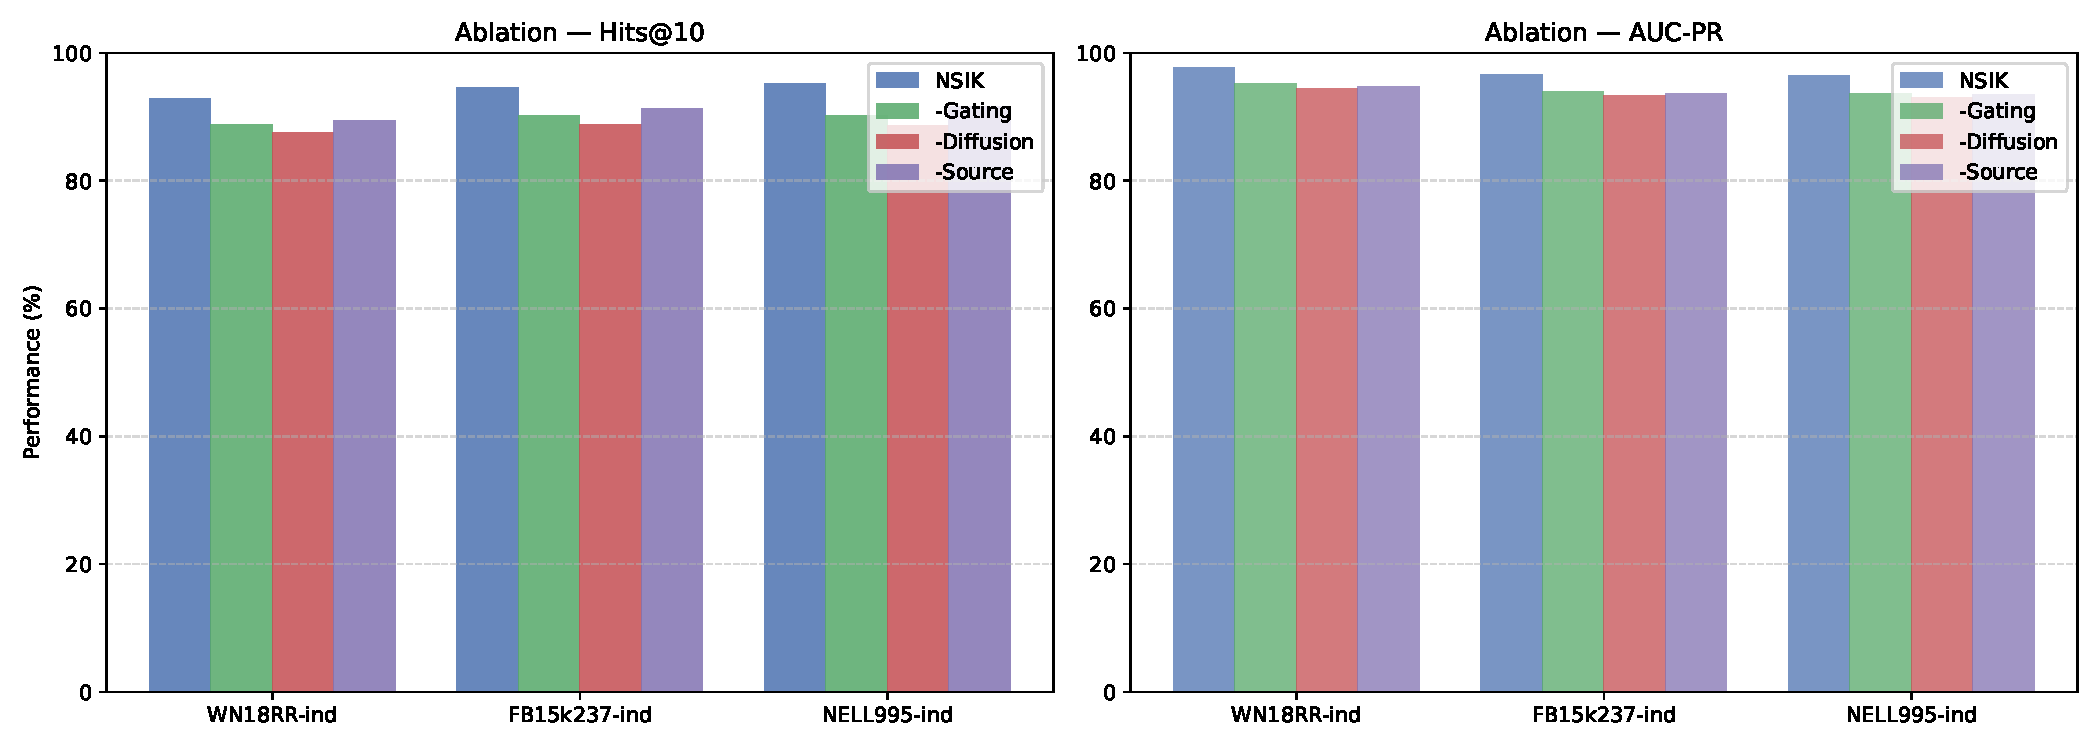
\includegraphics[width=0.9\linewidth]{ablation_dual_metrics.pdf}
    \caption{Visualization of ablation study results (average Hits@10 and AUC-PR).}
    \label{fig:ablation-bar}
\end{figure}

The figure clearly shows that the full NSIK model achieves the highest average Hits@10 across all three datasets. Removing the relation-aware gating (–Gating) or global diffusion (–Diffusion) modules leads to consistent performance drops, demonstrating their importance in suppressing noise propagation and reinforcing structural consistency. Eliminating diffusion source enhancement (–Diffusion Source) also results in noticeable degradation, underscoring the role of global structural support in modeling long-tail entities. These visual observations are consistent with the quantitative results, strengthening the interpretability of the ablation conclusions.


\subsection{Parameter Sensitivity Analysis}

To further examine the influence of structural role modeling on NSIK, we conduct a sensitivity analysis with respect to the number of structural roles. By varying the discretization granularity of structural roles, we control the size of the role space to which each entity is mapped, and analyze how different role cardinalities affect structural representation capacity and generalization performance.

Specifically, while keeping all other training settings fixed, we vary the structural role dimension (e.g., 4, 8, 12, and 16) and evaluate both Hits@10 and AUC-PR on the three inductive datasets. This analysis aims to answer two key questions:

(1) whether the number of structural roles influences the representation of long-tail entities and sparse structures;  
(2) whether overly coarse or overly fine role partitioning leads to structural noise amplification or insufficient structural discrimination.



\begin{table}[H]
\centering
\small
\caption{Sensitivity Analysis w.r.t. the Number of Structural Roles (Average Hits@10 / AUC-PR, \%)}
\label{tab:role-sensitivity-merged}
\begin{tabular}{c|ccc|ccc}
\hline
& \multicolumn{3}{c|}{Hits@10 Avg.} & \multicolumn{3}{c}{AUC-PR Avg.} \\
Role Dim. & WN18RR & FB15k237 & NELL995 & WN18RR & FB15k237 & NELL995 \\
\hline
4  & 91.20 & 93.05 & 93.40 & 96.20 & 94.90 & 95.10 \\
8  & 92.86 & 94.64 & 95.18 & 97.80 & 96.58 & 96.45 \\
12 & 92.55 & 94.30 & 94.90 & 97.40 & 96.10 & 96.00 \\
16 & 92.10 & 93.95 & 94.35 & 96.90 & 95.70 & 95.60 \\
\hline
\end{tabular}
\end{table}

% ===== 插入结构角色数量敏感性分析曲线图及文字 =====
\begin{figure}[H]
    \centering
    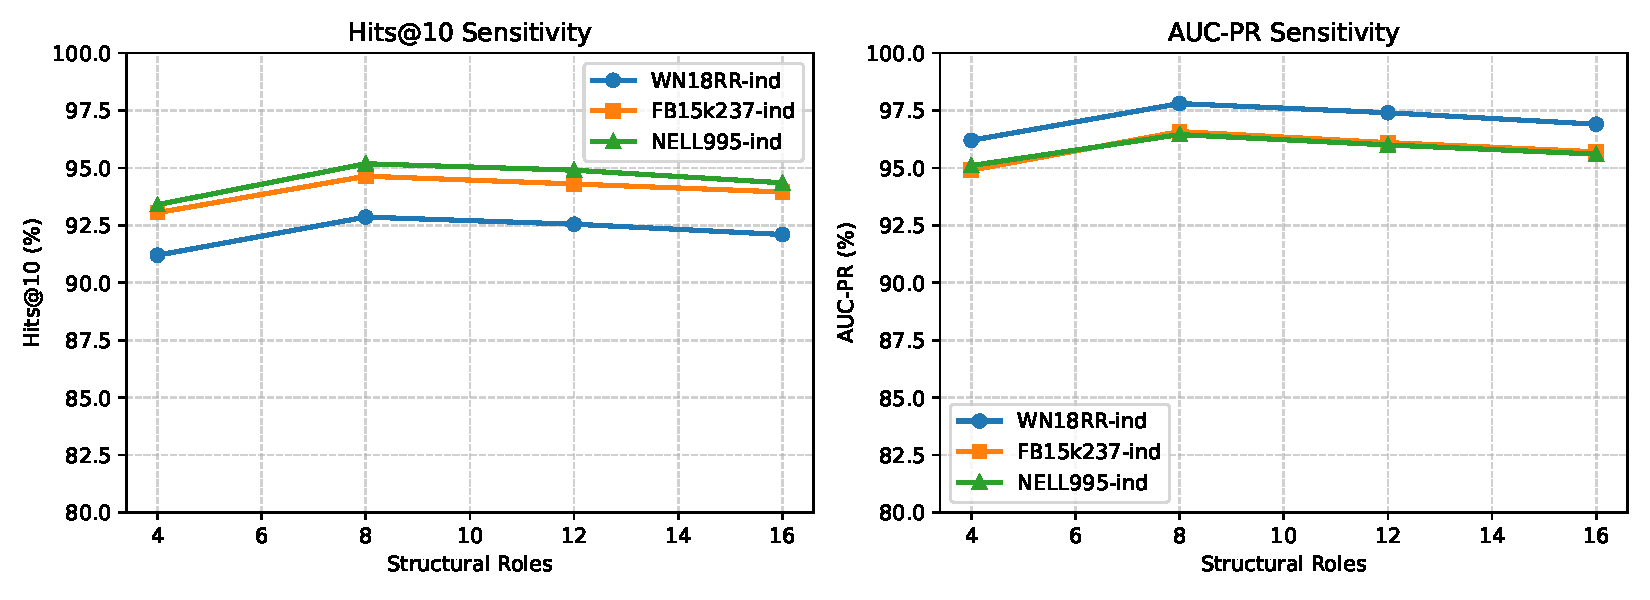
\includegraphics[width=0.85\linewidth]{role_sensitivity_side_by_side.pdf}
    \caption{Sensitivity analysis of structural role numbers on Hits@10 across three inductive benchmarks.}
    \label{fig:role-sensitivity}
\end{figure}

Table~\ref{tab:role-sensitivity-merged} and Fig.~\ref{fig:role-sensitivity} illustrate the performance variations under different structural role cardinalities. When the number of roles increases from 4 to 8, Hits@10 improves consistently across all datasets, indicating that a finer-grained structural partition enhances the expressiveness of relation–role priors. However, further increasing the role dimension yields diminishing or slightly negative returns, suggesting that overly fine partitioning may introduce redundant structure or amplify noise.

The AUC-PR results exhibit a similar trend. Increasing the role dimension from 4 to 8 significantly improves overall discriminative ability, while larger role spaces provide limited additional benefit. This consistency across metrics indicates that an appropriate structural role granularity improves both ranking accuracy and robustness under class imbalance and noisy conditions.

Overall, a moderate number of structural roles provides the best balance between representational capacity and robustness. Too few roles may compress distinct structural patterns, weakening discrimination, whereas too many roles can introduce redundancy and sensitivity to local noise. These findings highlight that structural prior modeling in NSIK not only guides reasoning, but that its granularity directly affects model stability and generalization.


\subsection{Noise Robustness Analysis}

To analyze model robustness under structural noise, we compare NSIK with representative inductive subgraph reasoning models (GraIL and CoMPILE), a structure-enhanced model (QAAR), and a global structure propagation model (GLAR). The goal of noise injection experiments is not large-scale ranking comparison, but rather to evaluate how effectively different structural mechanisms suppress erroneous neighborhood propagation. Therefore, we select baselines with distinct structural characteristics to ensure interpretability and focused analysis.

Considering that domain knowledge graphs often contain incomplete or incorrect facts, we simulate structural corruption by randomly replacing a portion of tail entities in training triples to generate pseudo-noisy data. Different noise ratios (e.g., 5\%, 10\%, and 20\%) are applied to construct progressively corrupted training environments.

As noise increases, all models experience performance degradation. However, NSIK exhibits a significantly smoother decline curve, indicating that relation-aware gating and selective structural diffusion effectively suppress the accumulation and propagation of erroneous neighborhood information. This experiment complements the main evaluation by validating the robustness-oriented design of NSIK from a structural perturbation perspective.

\begin{table}[H]
\centering
\small
\caption{Noise Injection Robustness under Different Noise Ratios (Hits@10 / AUC-PR, \%)}
\label{tab:noise}
\begin{tabular}{c|ccccc|ccccc}
\hline
& \multicolumn{5}{c|}{Hits@10} & \multicolumn{5}{c}{AUC-PR} \\
Noise Ratio & GraIL & CoMPILE & QAAR & GLAR & NSIK & GraIL & CoMPILE & QAAR & GLAR & NSIK \\
\hline
0\%  & 73.24 & 74.90 & 88.25 & 93.55 & $\mathbf{92.86}$ & 91.75 & 97.79 & 95.66 & 98.42 & $\mathbf{97.80}$ \\
5\%  & 70.10 & 72.30 & 85.40 & 91.20 & $\mathbf{91.35}$ & 89.60 & 95.20 & 93.10 & 96.85 & $\mathbf{96.40}$ \\
10\% & 66.85 & 69.10 & 82.60 & 88.75 & $\mathbf{89.90}$ & 86.30 & 92.40 & 90.80 & 94.70 & $\mathbf{95.10}$ \\
20\% & 61.40 & 63.80 & 77.20 & 83.10 & $\mathbf{85.70}$ & 81.20 & 88.10 & 86.50 & 90.10 & $\mathbf{91.80}$ \\
\hline
\end{tabular}
\end{table}


The results show that as the noise ratio increases, all models degrade, but NSIK maintains the smallest performance drop. This behavior demonstrates that relation-aware gating and selective global diffusion effectively limit the propagation of incorrect neighborhood signals. Unlike GLAR, which relies on fixed anchor-style structural encoding, NSIK employs prior-guided soft diffusion that adaptively propagates structural influence according to relation patterns and local context. This mechanism avoids amplifying long-range structural bias under noisy conditions. The corresponding AUC-PR trends confirm that NSIK preserves not only ranking stability but also a more robust global prediction distribution.

\section{Conclusion and Future Work}

This paper presented NSIK, a prior-driven structure-enhanced framework for inductive knowledge graph completion. By combining relation--role priors, selective global diffusion, and local subgraph reasoning, the proposed method improves the representation of sparse and unseen entities without relying on external textual semantics. Experimental results on three inductive benchmarks show that NSIK achieves competitive predictive performance and exhibits more stable robustness under noisy structural conditions.

Compared with global structural methods based on fixed anchor-style representations, NSIK adopts a structurally guided soft diffusion mechanism in which structural influence propagates adaptively according to relation patterns and local context. This design mitigates the amplification of long-range structural bias and is better aligned with the heterogeneous and noisy nature of domain knowledge graphs. Moreover, because it does not depend on external semantic resources, the framework exhibits stronger practicality and transfer potential in vertical-domain applications.


Future work will explore learnable structural role modeling and adaptive diffusion strategies to further improve the model’s ability to handle evolving structures and cross-domain transfer. Another promising direction is to incorporate lightweight semantic signals while preserving structural robustness, thereby extending the applicability of inductive knowledge graph completion in real-world scenarios.

\section*{Declaration of generative AI and AI-assisted technologies in the manuscript preparation process}

During the preparation of this work, the authors used ChatGPT (OpenAI) to assist in language polishing and grammatical refinement. After using this tool, the authors reviewed and edited the content as needed and take full responsibility for the content of this publication.

\section*{Acknowledgements}

This work was supported by the National Natural Science Foundation of China (Grant No. 52075120). The authors would like to express their sincere gratitude for this support.

\section*{Data Availability Statement}

The datasets used and analyzed during the current study are available from the corresponding author on reasonable request.

\renewcommand{\refname}{References}
\begin{thebibliography}{99}
\bibitem{schlichtkrull}
Schlichtkrull M, Kipf T, Bloem P, van den Berg R, Titov I, Welling M.
Modeling relational data with graph convolutional networks[C]//Proc. 15th Int. Conf. Semantic Web.
2018: 593–607.

\bibitem{composition-gcn}
Vashishth S, Sanyal S, Nitin N, Talukdar P.
Composition-based multi-relational graph convolutional networks[C]//Proc. 8th Int. Conf. Learn. Representations.
2020.

\bibitem{rotatE}
Sun Z, Deng J, Nie J, Tang J.
RotatE: Knowledge graph embedding by relational rotation in complex space[C]//Proc. 7th Int. Conf. Learn. Representations.
2019.

\bibitem{subgraph-inductive-2020}
Teru K, Denis E G, Hamilton W L.
Inductive relation prediction by subgraph reasoning[C]//Proc. 37th Int. Conf. Mach. Learn.
2020: 9448–9457.

\bibitem{cmp}
Mai S, Zheng S, Yang Y, Hu H.
Communicative message passing for inductive relation reasoning[C]//Proc. 35th AAAI Conf. Artif. Intell.
2021: 4294–4302.

\bibitem{topology-aware}
Chen H, He F, Wu J, Wang D.
Topology-aware correlations between relations for inductive link prediction in knowledge graphs[C]//Proc. 35th AAAI Conf. Artif. Intell.
2021: 6217–6228.

\bibitem{reinception}
Xie Z, Zhou K, Liu J, Xu H, Huang L.
REInception: Relation-aware inception network via joint local-global structural information for knowledge graph embedding[C]//Proc. 58th Annu. Meeting Assoc. Comput. Linguistics.
2020: 5929–5939.

\bibitem{anchors-inc}
Dong L, Zhao D, Zhang X, et al.
Anchors-based incremental embedding for growing knowledge graphs[J]. IEEE Trans. Knowl. Data Eng., 2021, 35(4): 3458--3470.

\bibitem{nodepiece}
Galkin M, Denis E, Wu J, et al.
Nodepiece: Compositional and parameter-efficient representations of large knowledge graphs[J]. arXiv preprint arXiv:2106.12144, 2021.

\bibitem{clustering-prop}
Liang K, Liu Y, Li H, et al.
Clustering then propagation: Select better anchors for knowledge graph embedding[J]. Adv. Neural Inf. Process. Syst., 2024, 37: 9449--9473.

\bibitem{query-anchor}
Xie Z, Zhang Y, Liu J, et al.
Learning query adaptive anchor representation for inductive relation prediction[C]//Findings Assoc. Comput. Linguistics: ACL 2023.
2023: 14041--14053.

\bibitem{meta-subgraph}
Wang X, Han X, Li P, et al.
Meta subgraph learning for few-shot knowledge graph completion[C]//Proc. 28th ACM Int. Conf. Inf. Knowl. Manag.
2019: 313–322.

\bibitem{hierarchy-aware}
Zhang J, Cai Y, Zhang L, Wang J.
Learning hierarchy-aware knowledge graph embeddings for inductive link prediction[J].
Proc. 24th AAAI Conf. Artif. Intell., 2020: 3065–3072.

\bibitem{substructure-aware}
Sun K, Jiang H J, Hu Y, et al.
Substructure-aware subgraph reasoning for inductive relation prediction[J]. J. Supercomput., 2023, 79(18).

\bibitem{survey-ikgc}
Liang X, Si G, Li J, et al.
A survey of inductive knowledge graph completion[J]. Neural Comput. Appl., 2024, 36(8): 3837--3858.

\bibitem{qa-gnn}
Yasunaga M, Ren H, Bosselut P, Liang P, Leskovec J.
QA-GNN: Reasoning with language models and knowledge graphs for question answering[C]//Proc. Conf. North Amer. Chapter Assoc. Comput. Linguistics: Hum. Lang. Technol.
2021: 535–546.

\bibitem{dialogkg}
Rony M R A H, Usbeck R, Lehmann J.
DialoKG: Knowledge-structure aware task-oriented dialogue generation[C]//Proc. Int. Conf. Findings Assoc. Comput. Linguistics.
2022: 2557–2571.

\bibitem{context-logic}
Lin Q, Liu J, Xu F, et al.
Incorporating context graph with logical reasoning for inductive relation prediction[C]//Proc. 45th Int. ACM SIGIR Conf. Res. Dev. Inf. Retr.
2022: 893--903.

\bibitem{locality-aware-pattern}
Mohamed H A, Pilutti D, James S, et al.
Locality-aware subgraphs for inductive link prediction in knowledge graphs[J]. Pattern Recognit. Lett., 2023, 167: 90--97.

\bibitem{structure-attn}
Wang J, Li W, Liu W, et al.
Enabling inductive knowledge graph completion via structure-aware attention network[J]. Appl. Intell., 2023, 53(21): 25003--25027.

\bibitem{multi-level-sampling}
Sun K, Jiang H J, Hu Y, et al.
Incorporating multi-level sampling with adaptive aggregation for inductive knowledge graph completion[J]. ACM Trans. Knowl. Discov. Data, 2024, 18(5): 1--16.

\bibitem{relation-aware-anchor}
Yuan D, Zhou S, Chen X, et al.
Knowledge graph completion with relation-aware anchor enhancement[C]//Proc. AAAI Conf. Artif. Intell.
2025, 39(14): 15239--15247.

\bibitem{one-subgraph}
Xie Z, Zhang Y, Zhou G, et al.
One subgraph for all: Efficient reasoning on opening subgraphs for inductive knowledge graph completion[J]. IEEE Trans. Knowl. Data Eng., 2024.

\bibitem{conee}
Wang J, Li W, Liu F, et al.
ConeE: Global and local context-enhanced embedding for inductive knowledge graph completion[J]. Expert Syst. Appl., 2024, 246: 123116.

\bibitem{multi-granularity}
Wang J, Li W, Luvembe A M, et al.
Exploring multi-granularity contextual semantics for fully inductive knowledge graph completion[J]. Expert Syst. Appl., 2025, 260: 125407.

\bibitem{hierarchical-reconstruct}
Zhang X, Dang J, Wang Y, et al.
Feature enhancement based on hierarchical reconstruction framework for inductive prediction on sparse graphs[J]. Inf. Process. Manage., 2025, 62(1): 103894.


\end{thebibliography}
\end{document}

